\section{HSL}
\subsection{Introducción}
\textit{HSL} es un filtro que consta de tres etapas:
\begin{enumerate}
\item \textbf{RGBtoHSL:} consiste en un cambio del espacio de color de los pixeles, desde RGB a HSL. 
\item \textbf{Suma:} se procesan los píxeles sumándole valores pasados por parámetro a cada una de las componentes.
\item \textbf{RGBtoHSL:} se realiza la operación inversa a la de la primera etapa, es decir, el pasaje del espacio HSL a RGB.
\end{enumerate}

El pseudocódigo de cada una de estas etapas es descripto en el enunciado del TP.

\subsection{Implementación 1}
En esta sección se pide realizar una implementación de la etapa de \textit{Suma} en ASM y desde la misma llamar a las funciones en C para convertir entre RGB y HSL.\\
Como las funciones \textit{RGBtoHSL} y \textit{hslTOrgb} procesan de a un pixel, es necesario iterar sobre cada pixel de la imagen para para ir procesándolos.\\

De esta forma, los pasos que se realizan en una iteración del ciclo son los siguientes:

\begin{enumerate}

\item Tomar un pixel de la imagen.
\item Llamar a la función \textit{RGBtoHSL} de C.
\item Con el pixel ya transformado al espacio HSL, hay que realizar la operación de suma en sí. Esta se realiza de la siguiente manera:\\

\textbf{Pseudocódigo de Suma}
\begin{verbatim}
	if( h+HH >= 360 ) h = h + HH - 360
	else if( h+HH < 0 ) h = h + HH + 360
	else
	    h = h + HH
	if( s+SS >= 1 ) s = 1
	else if( s+SS < 0 ) s = 0
	else
	    s = s + SS
	if( l+LL >= 1 ) l = 1
	else if( l+LL < 0 ) l = 0
	else
	    l = l + LL         
\end{verbatim}
Para poder realizar estas operaciones, necesitamos armar un registro de que contenga cuatro dwords que tengan la siguiente forma:

\begin{tabular}{| g | g | g | g |} %tabla color orange
\hline
$l+LL$ & $s+SS$ & $h+HH$ & $aa$ \\ 
\hline
\end{tabular}

Donde \textit{h}, \textit{s} y \textit{l} son las componentes del pixel HSL y \textit{HH}, \textit{SS} y \textit{LL} los valores pasados como parámetros. El \textit{aa} es el dword correspondiente al alfa, que va a quedar sin modificaciones.

Para realizar el registro mostrado anteriormente realizamos las siguientes operaciones:

\begin{lstlisting}
movss xmm1, [posicion_de_memoria_donde_esta_LL]	;xmm1 = |00|00|00|LL|
pslldq xmm1, 12			;xmm1 = |00|00|LL|00| - shift a izquierda
movss xmm2, [posicion_de_memoria_donde_esta_SS]	;xmm1 = |00|00|LL|SS|
pslldq xmm2, 8			;xmm1 = |00|LL|SS|00| - shift a izquierda
movss xmm3, [posicion_de_memoria_donde_esta_HH]	;xmm1 = |00|LL|SS|HH|
pslldq xmm3, 4			;xmm1 = |LL|SS|HH|aa| - shift a izquierda
\end{lstlisting}
Y luego, sumamos este registro al registro en donde tenemos a los tres componentes HSL de pixel.\\ Llamaremos a este registro \textit{origen} para claridad.

Estas operaciones debemos realizarlas en cada iteración del ciclo, porque tras el llamado a funciones de C, la convención no nos asegura que los registros XMM mantendrán sus valores.\\
Por último en este paso, vamos a armar las máscaras que necesitamos para realizar las operaciones del pseudocódigo que mostramos al principio de este punto.\\
Realizamos los siguientes defines:\\
\begin{verbatim}
comparar: dd 0.0, 360.0, 1.0, 1.0
vuelta_atras: dd 0.0, -360.0, 1.0, 1.0
vuelta_adelante: dd	0.0, 360.0, 0.0, 0.0         
\end{verbatim}
Y preparamos los siguientes registros:
\begin{lstlisting}
;traigo mascaras
	movups xmm10, [comparar]
	pxor xmm11, xmm11	;llamaremos ceros a xmm11
	movups xmm2, [vuelta_atras]
	movups xmm3, [vuelta_adelante]

;preparo datos con mascaras
	pxor xmm5, xmm5
	movlhps xmm5, xmm0	;xmm5 = |h+HH|aa|00|00|
	psrldq xmm5, 8			;xmm5 = |00|00|h+HH|aa|
	movups xmm6, xmm5		;xmm6 = |00|00|h+HH|aa|
	addps xmm5, xmm2		;xmm5 = |1|1|h+HH-360|aa| - llamaremos resultadoTRUEif a xmm5
	addps xmm6, xmm3		;xmm6 = |0|0|h+HH+360|aa| - llamaremos resultadoFALSEif a xmm6

\end{lstlisting}

\item En el punto anterior preparamos todos los registros necesarios para finalmente en este punto, realizar la lógica de suma según el pseudocódigo visto.\\
Como las componentes están enpaquetadas, debemos realizar las comparaciones simultáneamente. Para esto nos valemos de las máscaras que realizamos anteriormente. Para claridad al mostrar al código, reemplazaremos los registros efectivamente usados por los nombres de las etiquetas definidas en los defines y en los comentarios hechos anteriormente, donde armamos las máscaras necesarias.

\begin{lstlisting}
//xmm0, xmm1, xmm7 y xmm8 son copias de origen.
;if h+HH>=360 || s+SS>1 || l+LL>1
	cmpps xmm0, comparar, 5	;5 = greater equal
	pand xmm0, resultadoTRUEif

;if 0<=h+HH<360 || 0<=s+SS<1 || 0<=l+LL<1
	cmpps xmm7, comparar, 1	;1 = less than
	cmpps xmm8, ceros, 5	;5 = greater equal - ceros es un registro con ceros hecho con un pxor entre un registro XMM y si mismo.
	pand xmm7, xmm8
	pand xmm7, xmm1

;if h+HH<0 || s+SS<0 || l+LL<0
	cmpps xmm1,	xmm11, 1	;1 = less than
	pand xmm1, resultadoFALSEif

;sumo todos los valores con las mascaras aplicadas
	por xmm0, xmm7
	por xmm0, xmm1
\end{lstlisting}
En este punto tenemos en xmm0 el resultado para cada componente tras realizar las comparaciones indicadas por el pseudocódigo y asignar el valor indicado en cada caso. 
\item Con el pixel ya modificado en todas sus componentes, ahora ya podemos pasarselo a la función \textbf{hslTOrgb} para volver a pasar al espacio RGB.
\item Finalmente, avanzamos un pixel y volvemos a iterar.

\end{enumerate}

\subsection{Implementación 2}
La consigna en esta implementación es desarrollar todas las etapas del filtro en ASM.\\
De esta manera, para la etapa de \textit{Suma} se aprovechó la implementación anterior y se desarrolló en Assembler las etapas restantes. Es decir, ahora tendremos la conversión RGB a HSL y HSL a RGB en dos rutinas separadas, programadas en Assembler.\\

Al igual que en la primer implementación, se procesó de a un pixel por vez.\\

Para la primer conversión (\textit{RGB to HSL}) se busca el máximo y el mínimo de las componentes, y luego se comienza a definir $H$, $S$ y $L$.\\
Para definir $H$ se evaluaron los casos para donde cada compoente era la máxima, y en cada uno se realizo el proceso correspondiente indicado en el enunciado del trabajo. Luego se procesó el valor de $S$ y de $L$, y se devolvió a la rutina principal via el puntero a float recibido por parametro.\\

Para la segunda conversión (\textit{HSL to RGB}), primero se calculó el valor de $c$, $x$ y $m$, y luego se procedió a realizar el cálculo de $R$, $G$ y $B$. Para esto se uso la instrucciòn cmpss y algo de logica para hacer los distintos "ifs" necesarios.\\
Finalmente cargamos los resultados en el puntero a \textit{uint8\_t} pasado por parámetro y se retorna a la rutina principal.\\

\subsection{Resultados}
A continuación, mostraremos algunos de los resultados y conclusiones a los cuales llegamos a través de la experimentación de las distintas implementaciones según la estretegia ideada para este fin, detallada en la introducción.

Tener en cuenta que el porcentaje de desvío estándard para cada implementación de este filtro resultó ser de:
\begin{tabular}{| l | l |}
\hline
Implementación & Porcentaje de Desvío Estándard \\
HSL C	& $+/- +/- 3\%$\\
HSL ASM1 & 	$"+/- 6\%$\\
HSL ASM2	& $+/- 5\%$\\
\hline
\end{tabular}

Estos porcentajes representan que, para cada medición de cantidad de ciclos de clock de ejecución de una implementación dada de este filtro, tras descartar el 10\% de las peores mediciones, y tomar el promedio entre el 90\% de las mediciones restantes, el error varía entre +/- dicho porcentaje. Por ejemplo, dada la ejecución siguiente:

\begin{verbatim}
c hsl image_1_40x40.bmp salida.bmp 0.5 0.5 0.5
\end{verbatim}
Sobre las 100 repeticiones realizadas, tras descartar el 10\% de las peores, quedan 90 mediciones sobre las cuales el promedio calculado fue 209670 con margen de error de +/-3\%.\\

Las tablas a continuación representan, para cada implementación el promedio para las imágenes tendientes a un color determinado en cada uno de los distintos tamaños testeados. A su vez, en las últimas tres filas, se calcula el promedio general para dichos promedios, el desvío estandar entre ellos y el porcentaje de desvío.

\begin{tabular}{| l | l | l | l | l |}
\hline
Implementación & Color & 1600 píxeles & 90000 píxeles & 360000 píxeles\\
\hline
Hsl ASM1 0.5 0.5 0.5 & azul & 359764.53 & 18520763.60 & 72633855.47\\ 
\hline
Hsl ASM1 0.5 0.5 0.5 & blanco & 310855.33 & 18855768.67 & 70170817.33\\ 
\hline
Hsl ASM1 0.5 0.5 0.5 & mixto & 327535.44 & 18280896.22 & 72698313.33\\ 
\hline
Hsl ASM1 0.5 0.5 0.5 & negro & 223275.25 & 12070519.50 & 49497420.00\\
\hline
Hsl ASM1 0.5 0.5 0.5 & rojo & 329826.75 & 17855115.50 & 69956707.00\\
\hline
Hsl ASM1 0.5 0.5 0.5 & verde & 315792.50 & 18595604.50 & 71852216.00\\ 
\hline
Promedio & &  311174.97 & 17363111.33 & 67801554.86\\
\hline
Desvio estándard  && 46312.60 & 2614695.00  & 9044740.65\\
\hline
Porcentaje de desviación  && 14.88\% & 15.06\% & 13.34\%\\
\hline
\end{tabular}

\begin{tabular}{| l | l | l | l | l |}
\hline
Implementación & Color & 1600 píxeles & 90000 píxeles & 360000 píxeles\\
\hline
Hsl ASM2 0.5 0.5 0.5 & azul & 284234.93 & 12611483.33 & 50635606.13\\ 
\hline
Hsl ASM2 0.5 0.5 0.5 & blanco & 284863.67 & 13172857.33 & 50869777.33\\ 
\hline
Hsl ASM2 0.5 0.5 0.5 & mixto & 282192.78 & 13088796.78 & 50706775.56\\ 
\hline
Hsl ASM2 0.5 0.5 0.5 & negro & 233569.25 & 10897850.25 & 42586066.00\\
\hline
Hsl ASM2 0.5 0.5 0.5 & rojo & 291041.13 & 12736569.25 & 51346788.00\\
\hline
Hsl ASM2 0.5 0.5 0.5 & verde & 290393.00 & 12734652.00 & 51201397.00\\ 
\hline
Promedio & &  277715.79 & 12540368.16 & 49557735.00\\
\hline
Desvio estándard  &&  21912.68 & 834263.75 & 3426661.92\\
\hline
Porcentaje de desviación  &&  7.89\% &  6.65\% &  6.91\%\\
\hline
\end{tabular}

\begin{tabular}{| l | l | l | l | l |}
\hline
Implementación & Color & 1600 píxeles & 90000 píxeles & 360000 píxeles\\
\hline
Hsl C 0.5 0.5 0.5 & azul &  365585.53 & 16842125.00 & 64348957.33\\ 
\hline
Hsl C 0.5 0.5 0.5 & blanco & 377779.67 & 16876860.00 & 64668644.00\\ 
\hline
Hsl C 0.5 0.5 0.5 & mixto & 334989.89 & 16393089.44 & 64292180.89\\ 
\hline
Hsl C 0.5 0.5 0.5 & negro & 276944.25 & 11694642.25 & 46741104.00\\
\hline
Hsl C 0.5 0.5 0.5 & rojo &  350354.38 & 15877406.88 & 62859643.00\\
\hline
Hsl C 0.5 0.5 0.5 & verde &  360322.75 & 15394790.00 & 63306250.00\\ 
\hline
Promedio & &  344329.41 & 15513152.26 & 61036129.87\\
\hline
Desvio estándard  &&  36030.03  & 1955907.29 & 7037020.15\\
\hline
Porcentaje de desviación  && 10.46\% & 12.61\% &  11.53\%\\
\hline
\end{tabular}

A partir de éstas, confeccionamos la siguiente tabla que luego graficamos, utilizando escala logarítmica, para poder evaluar cómo era el rendimiento en promedio de las tres implementaciones en los distintos tamaños de imágenes.\\

\begin{tabular}{| l | l | l | l|}
\hline
Implementación	& 1600 píxeles & 90000 píxeles & 360000 píxeles\\
\hline
Hsl ASM1 0.5 0.5 0.5	& 311174.96	& 17363111.33 & 	67801554.85\\
\hline
Hsl ASM2 0.5 0.5 0.5	& 277715.79	& 12540368.15	& 49557735.00\\
\hline
Hsl C 0.5 0.5 0.5	& 344329.41	& 15513152.26	& 61036129.87\\
\hline
\end{tabular}

\begin{figure}[ht]
\centering
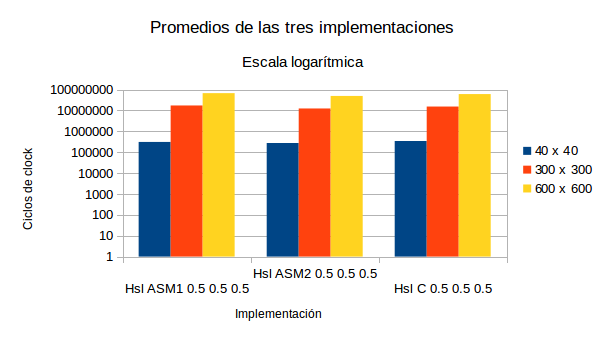
\includegraphics[width=90mm]{hsl/graficoHsl.png}
%\caption{A simple caption \label{overflow}}
\end{figure}

A continuación, mostraremos las tablas correspondientes a las imágenes de tipo "color constante", es decir, imágenes puramente rojas, verdes, azules, blancas y negras, que tratamos por separado para evaluar si registraban un comportamineto distinto.\\

\begin{tabular}{| l | l | l | l | l |}
\hline
Implementación & Color & 1600 píxeles & 90000 píxeles & 360000 píxeles\\
\hline
Hsl ASM1 0.5 0.5 0.5 & Uniforme Blanca & 231075.00 & 10941995.00 & 41332836.00\\ 
\hline
Hsl ASM1 0.5 0.5 0.5 & Uniforme Negra & 233186.00 & 13472777.00 & 45535360.00\\ 
\hline
Hsl ASM1 0.5 0.5 0.5 & Uniforme Roja & 419964.00 & 18202474.00 & 74076088.00\\ 
\hline
Hsl ASM1 0.5 0.5 0.5 & Uniforme Verde & 392571.00 & 17789276.00 & 71168984.00\\
\hline
Hsl ASM1 0.5 0.5 0.5 & Uniforme Azul & 359244.00 & 17842096.00 & 72150072.00\\
\hline
Promedio & &  327208.00	& 15649723.60 & 60852668.00\\
\hline
Desvio estándard  &&  89420.35 & 3271181.78 & 16004376.86\\
\hline
Porcentaje de desviación  &&  27.33\% & 20.90\% & 26.30\%\\
\hline
\end{tabular}

\begin{tabular}{| l | l | l | l | l |}
\hline
Implementación & Color & 1600 píxeles & 90000 píxeles & 360000 píxeles\\
\hline
Hsl ASM2 0.5 0.5 0.5 & Uniforme Blanca & 261370.00 & 11202093.00 & 41456304.00\\ 
\hline
Hsl ASM2 0.5 0.5 0.5 & Uniforme Negra & 200118.00 & 10637117.00	& 40151872.00\\ 
\hline
Hsl ASM2 0.5 0.5 0.5 & Uniforme Roja & 09031.00	& 13109446.00 & 53225056.00\\ 
\hline
Hsl ASM2 0.5 0.5 0.5 & Uniforme Verde & 305518.00 & 12530113.00	& 51572832.00\\
\hline
Hsl ASM2 0.5 0.5 0.5 & Uniforme Azul & 292952.00 & 12556929.00 & 50722960.00\\
\hline
Promedio & &  273797.80	& 12007139.60 & 47425804.80\\
\hline
Desvio estándard  &&  45270.29	& 1038738.53	& 6128731.92\\
\hline
Porcentaje de desviación  &&  16.53\% & 	8.65\% & 	12.92\%\\
\hline
\end{tabular}

\begin{tabular}{| l | l | l | l | l |}
\hline
Implementación & Color & 1600 píxeles & 90000 píxeles & 360000 píxeles\\
\hline
Hsl C 0.5 0.5 0.5 & Uniforme Blanca & 204029.00	& 10340318.00 & 39518652.00\\ 
\hline
Hsl C 0.5 0.5 0.5 & Uniforme Negra & 233486.00	& 10644786.00 &	40521400.\\ 
\hline
Hsl C 0.5 0.5 0.5 & Uniforme Roja & 356866.00	& 16543328.00	& 63436016.00\\ 
\hline
Hsl C 0.5 0.5 0.5 & Uniforme Verde & 354434.00	& 15911884.00	& 62773144.00\\
\hline
Hsl C 0.5 0.5 0.5 & Uniforme Azul & 343594.00	& 16214899.00	& 61588924.00\\
\hline
Promedio & &  298481.80	& 13931043.00	& 53567627.20\\
\hline
Desvio estándard  &&  73688.97	& 3148672.47	& 12389971.63\\
\hline
Porcentaje de desviación  &&  24.69\%	& 22.60\% & 23.13\%\\
\hline
\end{tabular}

De manera análoga, tomando los promedios obtenidos, graficamos para poder comparar las performances de las implementaciones en estos casos.\\

\begin{tabular}{| l | l | l | l|}
\hline
Implementación	& 1600 píxeles & 90000 píxeles & 360000 píxeles\\
\hline
Hsl ASM1 0.5 0.5 0.5	& 327208	& 15649723.6	& 60852668\\
\hline
Hsl ASM2 0.5 0.5 0.5	&273797.8	& 12007139.6	& 47425804.8\\
\hline
Hsl C 0.5 0.5 0.5	& 298481.8	& 13931043	& 53567627.2\\
\hline
\end{tabular}


\begin{figure}[ht]
\centering
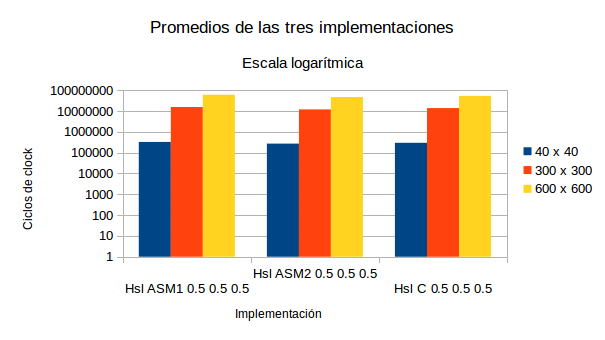
\includegraphics[width=90mm]{hsl/graficoHsl_cte.png}
%\caption{A simple caption \label{overflow}}
\end{figure}

\subsubsection{Algunas conclusiones}
Para HSL, la implementación más performante para los tres tamaños propuestos es ASM2, de la misma manera en que resultó ser para los otros filtros.\\
Dentro de cada implementación, como en los casos anteriores, los tiempos de ejecución evolucionan de manera creciente a medida que aumenta la cantidad de píxeles en las imágenes, lo cuál era lo que nos indicaba el sentido común.\\

Sin embargo, y tomando como estrategia de medición respecto de las diferencias entre los distintos tipos de imágenes la misma que la detallada en la introducción, los porcentajes de desvío estándar es mayor que en los otros filtros. Este resultado es en parte el esperado, ya que en esta implementación se toman acciones diferentes según el resultado que da sumar el color del pixel de la imagen al del parámetro recibido, entonces, es esperable que los tiempos de implementación divergieran en función de los distintos tipos de imágenes que tienden a distintos colores.\\

Sin tener en cuenta que las diferencias de performance en las distintas implementaciones de este ciclo se ven relacionadas con el uso de C o Assembler (en los distintos filtros se usa, o bien todo C, o bien mixto -implementación ASM1- o bien todo Assembler -en ASM2-), el punto anterior referente a la diferencia entre los tipos de imágenes es el más llamativo a la hora de evaluar la performance de las distintas implementaciones, a diferencia tal vez de los otros filtros implementados, en donde la desviación estándar en función de los tipos de imágenes era significativamente menor. 